\documentclass[11pt,a4paper]{article}
\usepackage[backend=bibtex]{biblatex}
\usepackage{graphicx}
\usepackage{siunitx}
\usepackage[mode=buildnew]{standalone}
\usepackage{subcaption}
\DeclareSIUnit\pixel{px}


\addbibresource{refs.bib}
\graphicspath{{./images}}

\newcommand{\convnet}{ConvNet}
\newcommand{\scatnet}{ScatNet}

\title{Comparison of \convnet and \scatnet}
\author{Edoardo Grassi}

\begin{document}
\maketitle



\section{Introduction}
% 1. Selezionare un dataset a scelta sul quale poi eseguire l’analisi per il progetto (da confermare poi con il docente)

The reference dataset for the project is the KTH-TIPS image dataset. The KTH-TIPS\cite{Fritz2004THEKD} (Textures under varying Illumination, Pose and Scale) image database was created to extend the CUReT database in two directions, by providing variations in scale as well as pose and illumination, and by imaging other samples of a subset of its materials in different settings. It contains 10 classes of material textures, shown in figure \ref{fig:samples}. Each sample from the dataset is preprocessed using the available support from the Torch library: the images are cropped and padded to match the common size of \qtyproduct{200x200}{\pixel}. The training phase is carried out on a subset of the dataset, namely a \SI{80}{\percent} split for the training and a \SI{20}{\percent} split for the validation.
%% TODO: is the dataset split actually balanced regarding class frequencies?

\begin{figure}\label{fig:samples}
    \includegraphics[width=0.8\textwidth]{dataset}
    \centering
    \caption{A sample for each class of the KTH-TIPS dataset}
\end{figure}


\section{ConvNet}
% 2. Implementare una CNN a piacere in pytorch
% 3. Classificare i dati grezzi. Visualizzare la matrice di confusione e da quest’ultima calcolare almeno 3 metriche per valutare la bontà delle classificazioni

The convolutional neural network ConvNet is based on the LeNet network architecture. The network performs feature extraction through convolutional layers and classification with a serie of fully connected layers.

\begin{figure}
    \label{fig:convnet:structure}
    \caption{Architecture of the ConvNet}
    % \includegraphics{convnet-structure}
    \includestandalone[page=1]{diagrams}
\end{figure}

\section{ScatNet}
% 4. Estrazione di feature tramite scattering e classificazione con lo stesso classificatore della CNN (es. MLP)

The model ScatNet uses a scattering layer to extract the set of features used for classification. The architecture of the network is summarized in figure \ref{fig:scatnet:structure}. The remaining network is composed of the classifier layers.

\begin{figure}\label{fig:scatnet:structure}
    \caption{Architecture of the ScatNet}
    % \includegraphics{scatnet-structure}
    \includestandalone[page=1]{diagrams}
\end{figure}

The underlying implementation of the scattering layer is provided by the python package \verb|kymatio|\cite{JMLR:v21:19-047} which offers a specific module for PyTorch which is compatible with the \verb|torch.nn.Module| interface. The scattering transform can be customized by some hyperparameters like the order $M$, the wavelet invariance scale $J$ and the rotations $L$.

The finalized model uses parameters $J=4$, $L=8$ and $M=2$\footnote{Package kimatio only supports scattering coefficients up to order $M=2$}. Given that the input shape of the dataset is $200 \times 200$, the feature vector resulting from the scattering layer has shape $100 \times 1$. The classifier architecture is the same one also used in the ConvNet network



\section{Results}
% 5. Confrontare i filtri estratti dallo scattering e i filtri della CNN

\begin{figure}[h]
    \label{fig:scatnet:confmat}
    \caption{Comparison of the resulting confusion matrices}
    
    \begin{subfigure}{0.5\textwidth}
        \includegraphics[width=\textwidth]{convnet-confmat}
        \caption{ConvNet}
    \end{subfigure}
    \hfill
    \begin{subfigure}{0.5\textwidth}
        \includegraphics[width=\textwidth]{scatnet-confmat}
        \caption{ScatNet}
    \end{subfigure}
\end{figure}

% \begin{figure}[h]
%     \label{fig:scatnet:metrics}
%     \caption{Metrics}
%     \begin{subfigure}{0.5\textwidth}
%         \includegraphics[width=\textwidth]{convnet-metrics}
%         \caption{ConvNet}
%     \end{subfigure}
%     \begin{subfigure}{0.5\textwidth}
%         \includegraphics[width=\textwidth]{scatnet-metrics}
%         \caption{ScatNet}
%     \end{subfigure}
% \end{figure}

\begin{figure}
    \label{fig:convnet:filters}
    \caption{Extracted filters from the convolution layers}
    \includegraphics{convnet-filters}
\end{figure}

\begin{figure}
    \label{fig:scatnet:filters}
    \caption{Filters}
    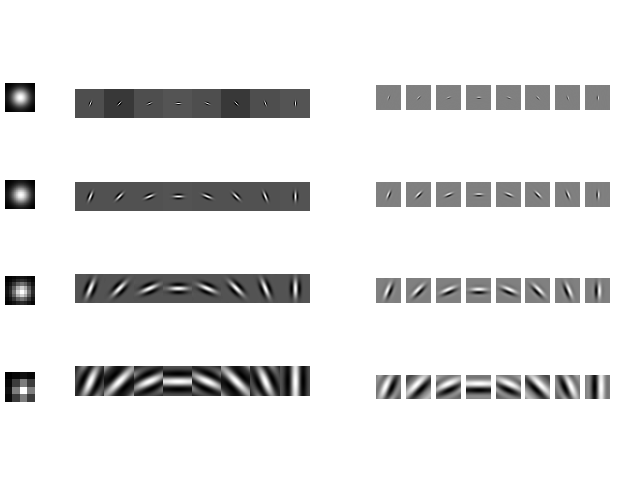
\includegraphics{scatnet-filters}
\end{figure}

\section{Analysis}
% 6. Commentare i risultati

Each model is scored with three classical metrics for ML tasks: accuracy, f1 score, and another one.

\printbibliography

\end{document}